\documentclass[a4paper,12pt]{report}

\usepackage[top = 1in, bottom = 1in, left = 1in, right = 1in]{geometry}
\usepackage{graphicx}
\usepackage{fancyhdr}
\usepackage{amsmath, amsthm, amssymb}
\usepackage{lastpage}
%\usepackage{subfigure}
\usepackage{lscape}
\usepackage{hyphenat}
\usepackage{setspace}
\usepackage{hyperref}  % used for \href and urls in .bib
\usepackage{xcolor}  % use to colour text
\usepackage{subfig}  % putting packages side by side
\usepackage{textcomp} % degree symbol

%\usepackage{listings}
\usepackage{pythonhighlight}
%\begin{python}
%x = 1
%\end{python}
%\pyth{__init__}


\usepackage{sectsty} % adjust size of chapter headings
\chapternumberfont{\large}
\chaptertitlefont{\Huge}

\usepackage{titlesec} % decrease the whitespace at chapter start
\titleformat{\chapter}[display]
{\normalfont\huge\bfseries}{\chaptertitlename\ \thechapter}{20pt}{\Huge}
\titlespacing*{\chapter}{0pt}{-40pt}{10pt}
%			{shift right/left}, {up/down}, {between title and text}

%%%%%%%%%%%%%%%%%%%%%%%%%%%%%%%%%%%%%%%%%%%%%%%%%%%%%%%%%%%%%%%%%%%%%%%%

% page formatting
\parskip = 6mm
\parindent = 0mm
\renewcommand{\headrulewidth}{0pt}
\rhead[]{\thesection}
\lhead[\thechapter]{}

%%%%%%%%%%%%%%%%%%%%%%%%%%%%%%%%%%%%%%%%%%%%%%%%%%%%%%%%%%%%%%%%%%%%%%%%

\begin{document}

\thispagestyle{empty}
{\Huge \begin{center}
Autonomous Object Identification and Tracking % title
\hrule
{\Large ya boi} % subtitle
\end{center}}

\vskip 5mm
\begin{center}

\includegraphics[scale = 0.3]{uctLogo.png}
\end{center}

\vskip 5mm
\begin{center}
Presented by:\\
Alexander Lutz Knemeyer
\end{center}

\vskip 10mm
\begin{center}
Prepared for:\\
Callen Fisher \\
Edward Boje \\
Dept. of Electrical and Electronics Engineering\\University of Cape Town
\end{center}

\vskip 10mm
\begin{center}
Submitted to the Department of Electrical Engineering at the University of Cape Town in partial fulfilment of the academic requirements for a Bachelor of Science degree in Mechatronics Engineering
\end{center}

\vskip 5mm
\begin{center}{\bf \today}
\end{center}

\newpage

%\thispagestyle{empty}  % leave a blank page
%\mbox{}
%\newpage

\onehalfspacing
\nohyphens{
\thispagestyle{empty}
\vskip 40mm

% Please leave the declaration as it is (Standard UCT declaration).
{\Large Declaration} \\
\hrule

\vskip 10mm
\begin{enumerate}
\item I know that plagiarism is wrong. Plagiarism is to use another's work and pretend that it is one's own.
\item I have used the IEEE convention for citation and referencing. Each contribution to, and quotation in, this report from the work(s) of other people has been attributed, and has been cited and referenced.
\item This report is my own work.
\item I have not allowed, and will not allow, anyone to copy my work with the intention of passing it off as their own work or part thereof.
\end{enumerate}

\vskip 10mm
Signature: \ldots\ldots\ldots\ldots\ldots\ldots\ldots\ldots\ldots
\\A. L. Knemeyer
\vskip10mm
Date: \ldots\ldots\ldots\ldots\ldots\ldots\ldots\ldots\ldots\ldots

\fancyfoot[C]{\thepage}
\pagestyle{plain}
\newpage

\pagenumbering{roman}
{\Large Acknowledgements} \\
\hrule

thanks Callen and Amir \\
thanks Sylv \\
thanks Justin Pead \\
thanks Stacey for laser cutting \\
thanks family and friends

\newpage

{\Large Abstract}\\
\hrule

% type a summary that identifies the purpose, problem, methods, results, and conclusion of your work

% [Explain the need/uses]
Many systems require a camera to autonomously identify the objects in its field of view, and then rotate the camera to keep it aimed at a certain class of object.

This report describes the design and implementation of such a system on a low-powered device. The system uses a Convolutional Neural Network to identify the position of objects from photos, making use of a neural accelerator device to achieve near real-time inferences. These measurements are improved through the use of a Kalman Filter, which estimates the angular state of the tracked object. A multiprocess pipeline is used to manage the control on a non-real time OS. Finally, a gimbal is designed and built to rotate the unique payload.

The tracking system is shown to have improvements over a stationary camera setup.

\newpage


\tableofcontents

\newpage
\listoffigures

\newpage
\listoftables


% Page formatting, to place section titles as headers of odd pages and Chapter titles as headers of even pages.
\newpage
\fancyhead[RE,LO]{}
\fancyhead[LE]{\leftmark}
\fancyhead[RO]{\rightmark}
\pagestyle{fancy}

\pagenumbering{arabic}

%%%%%%%%%%%%%%%%%%%%%%%%%%%%%%%%%%%%%%%%%%%%%%%%%%%%%%%%%%%%%%%%%%%%%%%%

\chapter{Introduction}
{\Large \color{red} have some text here? }
\section{Background to the study}

While the ability to autonomously track an object has a wide range of applications, it is useful to limit oneself to a particular need in order to produce quantifiable 'success or failure' metrics.

The UCT mechatronics laboratory's Rapid Acceleration and Manoeuvrability group studies cheetahs with the aim of reproducing their extraordinary manoeuvrability in two and four legged robots. For this, they require footage of cheetahs as they run. The cameras must be placed in pairs to achieve depth perception.

\vskip 15mm
{\Large \color{red} show top-down type image of multiple pairs of gopro cameras}
\vskip 15mm

Currently, they place multiple static pairs of cameras, each pair covering a different area, in order to continuously film an animal as it moves around. Having multiple cameras requires significant amounts of setup time, effort into synchronizing the footage, a total higher price as the cost of multiple cameras is expensive and extra work in keeping everything recharged. In addition, to maximise the time spent recording the animal, the cameras must be set to wide-angle. This introduces distortion into the recordings.


\section{Objectives of the study}
The objective of the study is thus to design and implement a system which can autonomously identify and track a fast-moving object using modern computer vision methods. A successful design would be cheaper overall, track the object for longer, and not require the cameras to be set to distorting wide-angle modes.


\section{Scope and limitations}
Due to the limited time and finances in an undergraduate thesis, the system will not be tested on actual cheetahs during the course of the project. Instead, it will be tested on humans and trained dogs with the hope that this sufficiently mimics the scenario of tracking cheetahs (or any other fast-moving object, for that matter).

However, the neural network will be retrained to be able to track cheetahs. This will be tested in simulation.

Finally, the study will be limited to tracking only one object in the frame at a time. This is because it is not immediately obvious what should be done when more than one object is present in the frame.


\section{Plan of development}
The development schedule was as follows:

\begin{enumerate}
\item Design the structure of the system as a whole.
\item Set up the main computing platform (a raspberry pi), installing relevant software and testing the camera module.
\item Choose a neural network architecture and deploy it onto the neural accelerator stick.
\item Design and 3D print a camera gimbal, and procure the necessary controller and actuators.
\item Rewrite the gimbal controller communication standard in python to allow the raspberry pi to send and receive commands.
\item Model the expected movement of the tracked object, and then design and implement a Kalman Filter (EKF).
\item Implement a parallel process-based data pipeline which takes a photo on the picam, preprocessess it, passes it through the neural accelerator, retrieves the results, passes the results into the EKF and then commands the gimbal motors to re-orient the camera appropriately.
\item Test final the system
\end{enumerate}

\section{Report outline}



\chapter{Literature Review}

\section{Importance and applications of ...}
this will be system-level stuff (general review of tracking objects) (will probably be centred around military and drone companies like DJI?) (also IR tracking, etc)

\section{Academic works related to ...}

\section{Computer vision using neural networks}
It was required that the system detect the position of an object from a photo. In particular, the object detector should,

\begin{itemize}
	\item Not require a beacon or light to be placed on the object,
	\item Run at around 5 to 10 Hz,
	\item Locate the object with high accuracy,
	\item Work regardless of the orientation of the object, and
	\item Be able to track any object with minimal extra work/design required.
\end{itemize}

This chapter details the literature sounding methods which could potentially achieve these requirements.

\subsection{Basic computer vision concepts}
Computer vision techniques tend to use a number of cascaded filters, with each layer of filters being able to detect more and more complex shapes in an image. These filters are known as 'kernels', and tend to be implemented as \pyth{3x3} matrices which are convolved with the input image, a 2D array of pixel values.

As an example, plotted below is an image before (left) and after (right) being convolved with a vertical line finding kernel.

\begin{figure}[h!]%
    \centering
    \subfloat{{
\includegraphics[width=3cm]{literature_review/input_image} }}%
    \qquad \qquad
    \subfloat{{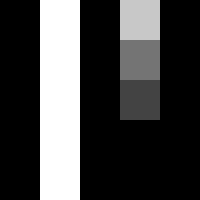
\includegraphics[width=3cm]{literature_review/output_image} }}%
    \caption{An image, before (left) and after (right) being convolved with a vertical line finder.}%
    \label{fig:example}%
\end{figure}

Note how the the vertical line in left part of the input has been found (represented by bright pixels in the output image). The horizontal line on the bottom right has been rejected. The faint vertical line in the top right has been found, albeit faintly. The exact same transformation is shown below, where the leftmost matrix is the input, the middle is the kernel and the rightmost matrix is the output.



\begin{table}[h!]
	\centering
	\begin{tabular}{ p{0.5cm} p{0.5cm} p{0.5cm} p{0.5cm} p{0.5cm} p{0.5cm} p{0.5cm} p{0.5cm} p{0.5cm} p{0.5cm} p{0.5cm} p{0.5cm} p{0.5cm} p{0.5cm} p{0.5cm}}
 5 & 232 & 180 & 212 & 180 &           &    &   &    &   & 0 & 255 & 0 & 200 & 0 \\
30 & 243 & 152 & 206 & 188 &           & -1 & 2 & -1 &   & 0 & 255 & 0 & 116 & 0 \\
32 & 255 & 210 & 190 & 190 & $\otimes$ & -1 & 2 & -1 & = & 0 & 255 & 67 & 0  & 0 \\
11 & 242 & 235 & 230 & 210 &           & -1 & 2 & -1 &   & 0 & 255 & 0 &  0  & 0 \\
90 & 240 & 130 &  20 &  30 &           &    &   &    &   & 0 & 255 & 0 &  0  & 0
	\end{tabular}
\end{table}

A larger, more interesting input image is shown below, in Figure~\ref{fig:image_kernel_demo}. The output image on the right hand side is the result of applying an edge-emphasizing filter. Note how the shape of the face and nose are highlighted.

\begin{figure}[h!]
  \centering
  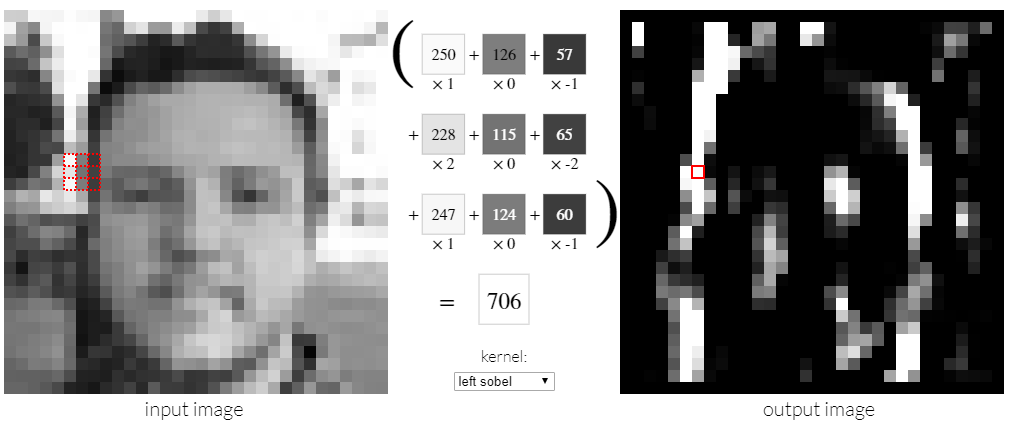
\includegraphics[width=\textwidth]{literature_review/image_kernel_demo}
  \caption{\label{fig:image_kernel_demo} A demonstration of image convolution on a photo of a human.}
\end{figure}

As an example of a complete system, the first layer of kernels may detect vertical lines, angled lines, dots, and so on. These detections are then used as input matrices to the next layer, which will convolve them with a set of kernels to produce more complex detections. For example, two horizontal lines and two vertical lines may indicate the presence of a square in an image. A different configuration of lines may indicate a circle, and so on.

Carefully designing and combining these filters can ultimately result in the detection of an object. However, this method is incredibly time consuming and requires extensive domain-specific knowledge. Even after the work has been put in to locate one type of object in a frame, locating another type of object may require the user to start from scratch.

\subsection{Introduction to machine learning}

Luckily, there exist other methods of creating and combining the kernels mentioned previously. Instead of hand-crafting each kernel and deciding how they should be combined, one could instead use machine-learning techniques (in which a computer can use a dataset of input-output pairs to learn the parameters of a model) to create kernels with 'optimal' values to find objects in a frame. This boils down to using data (known input-output pairs of an image of cheetah, and the label "cheetah") to optimize neural network.

The standard method of doing this for images is through the use of Convolutional Neural Networks (CNNs). CCNs are initialized with random values in their kernels and random weights which combine the outputs of their kernels - only their general architecture is fixed by human practitioners. The method to get accurate weights is then as follows:

\begin{enumerate}
\item Initialize the CNN with random values in the kernels and weights between 'neurons' (nodes in the CNN which perform an operation).
\item Pass an image through all the neurons in the CNN, and take note of the output.
\item Get the error (the difference between the CNN output and the correct answer) and propagate it back through the CNN, adjusting the weights \emph{slightly} in such a way that that same input would produce the correct output if run again.
\item Repeat the first three steps a few hundred or thousand times, using a large, diverse dataset.
\end{enumerate}

While it is possible that the CNN will act as a look-up table (mapping those specific inputs to their correct outputs, but giving the wrong result for any other dataset) it is hoped that the CNN will instead map any \emph{similar} input to the correct output. As an example, a correct training CNN will map any image which \emph{looks} like a cheetah (has the correct body structure, spots, ear location, etc) to an output which is numerically encoded to represent "cheetah".

It should be noted that CNNs are nothing more than a mapping from a vector of input pixels to a vector which represents certain outputs (such as "cheetah", "no cheetah" or even the coordinates of a cheetah).

CNNs simply require a few hundred or thousand labelled images and a few hours on a modern GPU. There are many open datasets which can be used to make this work easier.

\subsection{Key machine learning concepts and definitions}
Before getting lost in ReLU, dropout and the rest of the endless list of ideas in machine learning, it is worth considering the separation of jobs in in modern data science. Typically, there is one team which designs the neural network architecture, tunes hyper-parameters (import parameters usually set by humans), publishes results, and son on. This requires a certain set of skills.

Next, another person with a separate skill set puts the neural network in production in order to achieve some goal, possibly after training it them self. If you find yourself in the second group of people, you don't tend to need to keep up with every new paper published. Instead, armed with some understanding of the main innovations in each network design, you only need compare training techniques and architectures as a whole.

Since the project at hand doesn't necessitate a brand new architecture, only a handful ideas need to be discussed.

\textit{Machine learning, neural networks, deep learning, CNNs}: machine learning is the branch of computer science involved in fitting a model using data alone. Neural networks are a subset of machine learning, specifying a class of architectures loosely inspired by the synapses in the nervous system of an organic brain. Deep learning is the relatively recent practice of creating especially long neural networks in order to represent more complex mappings. Finally, CNNs are a subset of deep learning, in which the synapses of a deep neural network are kernels which perform convolution operations.

\textit{Image classification vs object detection:} an image classifier indicates \emph{what} object(s) are in an image. An object detector finds what objects are in the image, and also \emph{where} in the image they can be found. One might think to perform object detection using an image classification CNN by sliding the network over various overlapping parts of the input image, taking note of what part of the image the network is looking at when it finds an object - interestingly, this is almost exactly what object detectors do internally. In fact, it's exactly what convolution with a kernel does.

\textit{Bounding box: (or 'anchor'):} a pair of points which determine a box around a detected object.

\textit{Feature extractor:} it is common practice to concatenate an well-designed existing neural network with another architecture to produce a new, larger model which performs an overall more complex task. Thus, the role of the first part of the new model is to extract useful features for the second part to process.

\textit{Transfer learning:} this refers to the practice in which the weights of one neural network are copied to another network. This enables problems to be solved using much less data than neural networks ordinarily require, as the weights are already quite good before the retraining process. The idea is that the early layers are likely to have been trained to find very general features in the image (such as lines, circles, eyes, tails, etc). These are often relevant to a wide variety of problems. This is why a trained network will often have its training dataset specified - the content of the training dataset is a good indicator of whether transfer learning would help in a different problem.

\textit{Epoch:}

\textit{Batch size:}

\textit{Loss:}

\subsection{Movidius Neural Compute stick}
CNNs tend to require a large number of operations to produce an output. The exact amount of computation required depends on the neural network architecture, though even 'small' object detectors generally require on the order of millions of multiply-accumulate instructions with significant amounts of data being loaded to and from the various levels of cache. Combined with the slower processor on embedded computers such as a raspberry pi, the neural network would not be able to run in real time (inference time less than $\approx 100ms$). As an example, a cutting edge object detection network designed for use on mobile devices requires about 1 second to infer a result on the raspberry pi's CPU.

% nn and params: https://mxnet.apache.org/api/python/gluon/model_zoo.html

Fortunately, this work can be easily parallelised over multiple processing cores. There are three types of parallelization which tend to occur - during the application of kernels, during matrix multiplication and in parts of the neural network where the data flow is naturally parallel. This work is a perfect fit for GPUs, which contain a large number of processing cores designed for such tasks. However, since GPU support for CNNs on the raspberry pi is lacking, other means had to be investigated.

% https://petewarden.com/2014/08/07/how-to-optimize-raspberry-pi-code-using-its-gpu/
% https://rpiplayground.wordpress.com/2014/05/03/hacking-the-gpu-for-fun-and-profit-pt-1/

\textit{For the rest of this chapter, assume any obscure words have been patented by Intel$^{^{\ TM}}$ or one of its subsidiaries.}

To solve this problem, some chip makers have started to produce 'neural accelerators' - devices which can be used to decrease the inference time of neural network. One such as the Movidius Neural Compute Stick (NCS) - a specialized neural network accelerator which plugs into the raspberry pi (or any other computer). Its 12 purpose-built processing cores typically result in inference speed increases of between $700\%$ and $1000\%$. It also has the benefit of being purpose built for CNNs.

The operation of the Movidius NCS is as follows: first, the user designs and trains their neural network. Next, they compile it down to a device-specific format optimized for the NCS and upload it to the device. From then on, the user can send preprocessed images to the devices, wait for the inference to occur, and then retrieve the result.

The actual processing is done using Intel's Myriad 2 Vision Processing Unit (VPU), which makes use of 12 specially designed processing cores named 'shaves'.

%\begin{figure}[h!]
%  \centering
%  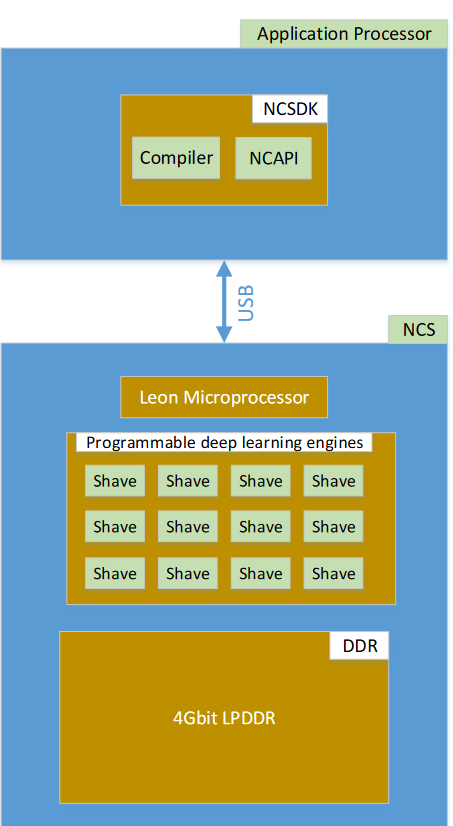
\includegraphics[width=0.4\textwidth]{literature_review/NCS_internals}
%  \caption{\label{fig:NCS_internals} Internals of the Movidius Neural Compute Stick.}
%\end{figure}


\subsection{Comparison of neural network architectures}
Not all neural network architectures are equal - generally, differences between models include,

\begin{itemize}
	\item Classification accuracy,
	\item Inference speed, which is a function of
	\begin{itemize}
		\item The number of operations (processing) and
		\item The number of weights (data retrieval)
	\end{itemize}
	\item The amount of data required for training/fine tuning,
	\item The existence (or lack) of pretrained models in each specific deep learning framework,
	\item Whether recent innovations in the field have been included, and
	\item The underlying method in which objects are detected and localised within the image
\end{itemize}

{\Large \color{red} COMPARE THIS STUFF!!! }

{\Large \color{red} MAYBE JUST LOOK AT THE AVAILABLE NETWORKS IN THE MOVIDIUS THING?}

Newer neural networks often take ideas from older architectures. Sometimes, they even include all or most of a previous architecture as part of the design of the new model. An example of this is MobileNet - an architecture designed at Google, aimed to run quickly on modern mobile devices (such as newer smartphones). A common practice is to train MobileNet to classify objects on a given dataset, then remove the final layers, concatenate it with another model (with MobileNet acting as a feature extractor) and end up with an object detector.

Since MobileNet was designed for mobile devices, it traded some classification accuracy for performance. However, the architecture is remarkable in that the performance increase is significant while the classification accuracy decrease is not.

Next was the choice of the actual object detector. There are two (TODO: check this) main ideas for this approach: one could get an image classifier and apply it to the image multiple times (such as 25 times) resulting in a grid of overlapping detections.

\section{The camera gimbal}
Once an object has been found and a desired control action calculated, the camera must be moved. This required the use of a camera gimbal which is powerful enough to rotate the payload specified by the researchers who will ultimately use the system: two GoPro Hero Session cameras, a distance sensor and the small camera used for tracking. Since this is a relatively unique payload, a new gimbal had to be designed and built. This chapter details the research which went into the design choices.

\subsection{An introduction to camera gimbals}
A gimbal is device which can rotate about one or more axis. A typical use is to place a camera and 3 actuators on a gimbal, resulting in the ability to rotate the camera in the roll, pitch and yaw axis. An annotated render of this can be found in Figure~\ref{fig:roll_pitch_yaw_camera}.

\begin{figure}[h!]
  \centering
  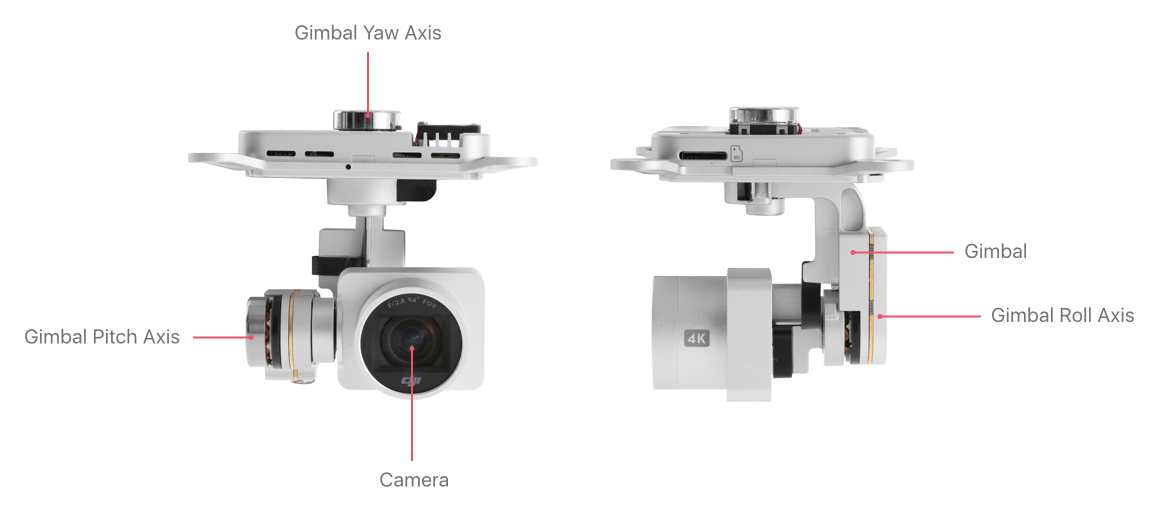
\includegraphics[width=\textwidth]{literature_review/roll_pitch_yaw_gimbal.png}
  \caption{\label{fig:roll_pitch_yaw_camera} An illustration of the roll, pitch and yaw axis used in a gimbal~\cite{roll_pitch_yaw_camera}.}
\end{figure}

While gimbal designs are \emph{fairly} standard, a few critical design choices must be made when building or buying one. The rest of this chapter will detail some of the options available.

\subsection{Comparison of actuator types}
The type of actuator used in the gimbal has a significant effect on the design of the gimbal, the speed it can move, the camera weight it can handle and quality of the resulting photos and videos. Thus, a few relevant actuator types were considered and compared. A summary of some of their relevant characteristics can be found below, in table \ref{table:gimbal_actuators}. Note that because there are a large number options for each actuator type, the metrics are generally more qualitative/comparative than strictly quantitative. The comparisons have been made for actuators which are of the size and cost required by the project, and available at local stores.
\newline

\begin{table}[h!]
	\centering
	\begin{tabular}{ p{2cm}||p{4cm}|p{4cm}|p{4cm} }
					& DC motor			& Servo motor		& BLDC \\
	\hline \hline
	Length			& $\approx 45mm$	& $\approx 50mm$	& $<30mm$ \\
	\hline
	Diameter		& $\approx 30mm$	& $50mm\times 20mm$	& $<30mm$ \\
	\hline
	Weight			& Moderate			& Heavier			& Light, requires ESC \\
	\hline
	Complexity		& Moderate (H-bridge) & Simple (built in) & Difficult (requires PID controller) \\
	\hline
	Circuitry required & H-bridge		& None (built in)	& Requires ESCs \\
	\hline
	Efficiency		& Low				& Low				& High \\
	\hline
	Maximum speed	& Low				& Low				& High \\
	\hline
	Price			& Low/moderate		& Low/moderate		& High \\
	\hline
	Smoothness		& Moderate			& Low				& Very high \\
	\hline
	\end{tabular}
	\caption{Comparison of gimbal actuators}
	\label{table:gimbal_actuators}
\end{table}

To summarize the main highlights from table \ref{table:gimbal_actuators}: DC motors are a poor choice for a system of this type because most options tend to be too long and heavy, or require complex gearing. Servo motors are not a good fit because, while they're easy to use (they're essentially a DC motor with circuitry built in) and have good torque, they're fairly large and tend to be quite jittery.

This leaves BLDC motors. While they can be quite complex to use and are somewhat expensive, they're compact, fast and tend to result in very smooth footage. As a result, they are the industry standard in camera gimbals. It is worth noting that, while the gimbal controller can be fairly complex, using a store-bought controller allows for one to easily leverage off the design work of other engineers. This results in a faster, smoother and more stable gimbal than one could build in a short period of time.

\subsection{\label{ssec:gimbal_design_inspirations}Gimbal design inspirations}
It is useful to review existing gimbal designs in order to avoid unnecessary re-invention of the wheel. Luckily, a large number of designs are available on the internet. One design which stood out from the research phase was \href{https://www.thingiverse.com}{thingiverse.com} member Velocirotor's clever gimbal design, dubbed the \href{https://www.thingiverse.com/thing:2804872}{Primbal Session} \cite{website:primbal_session}. It is light-weight, simple to 3D print and has an easy method to adjust length to balance the gimbal's three axis. A render of the design can be found in Figure~\ref{fig:primbal_pic}.

\begin{figure}[h!]
  \centering
  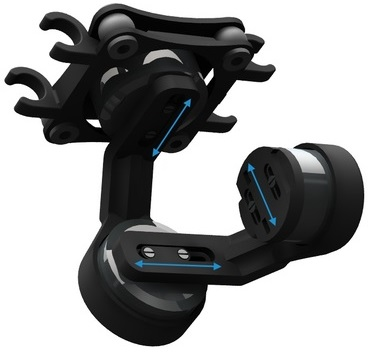
\includegraphics[width=0.5\textwidth]{literature_review/primbal_pic.jpg}
  \caption{\label{fig:primbal_pic} A render of the Primbal Session gimbal design.}
\end{figure}

Some inspiration was also taken from a gimbal designed by mechatronics engineering student Sylvan Morris, made during a period of vacation work. Noteworthy characteristics include the two-plate shock absorption system and method of mounting onto a quadcopter. A photo of his design can be found in Figure~\ref{fig:sylvan_gimbal}.

\begin{figure}[h!]
  \centering
  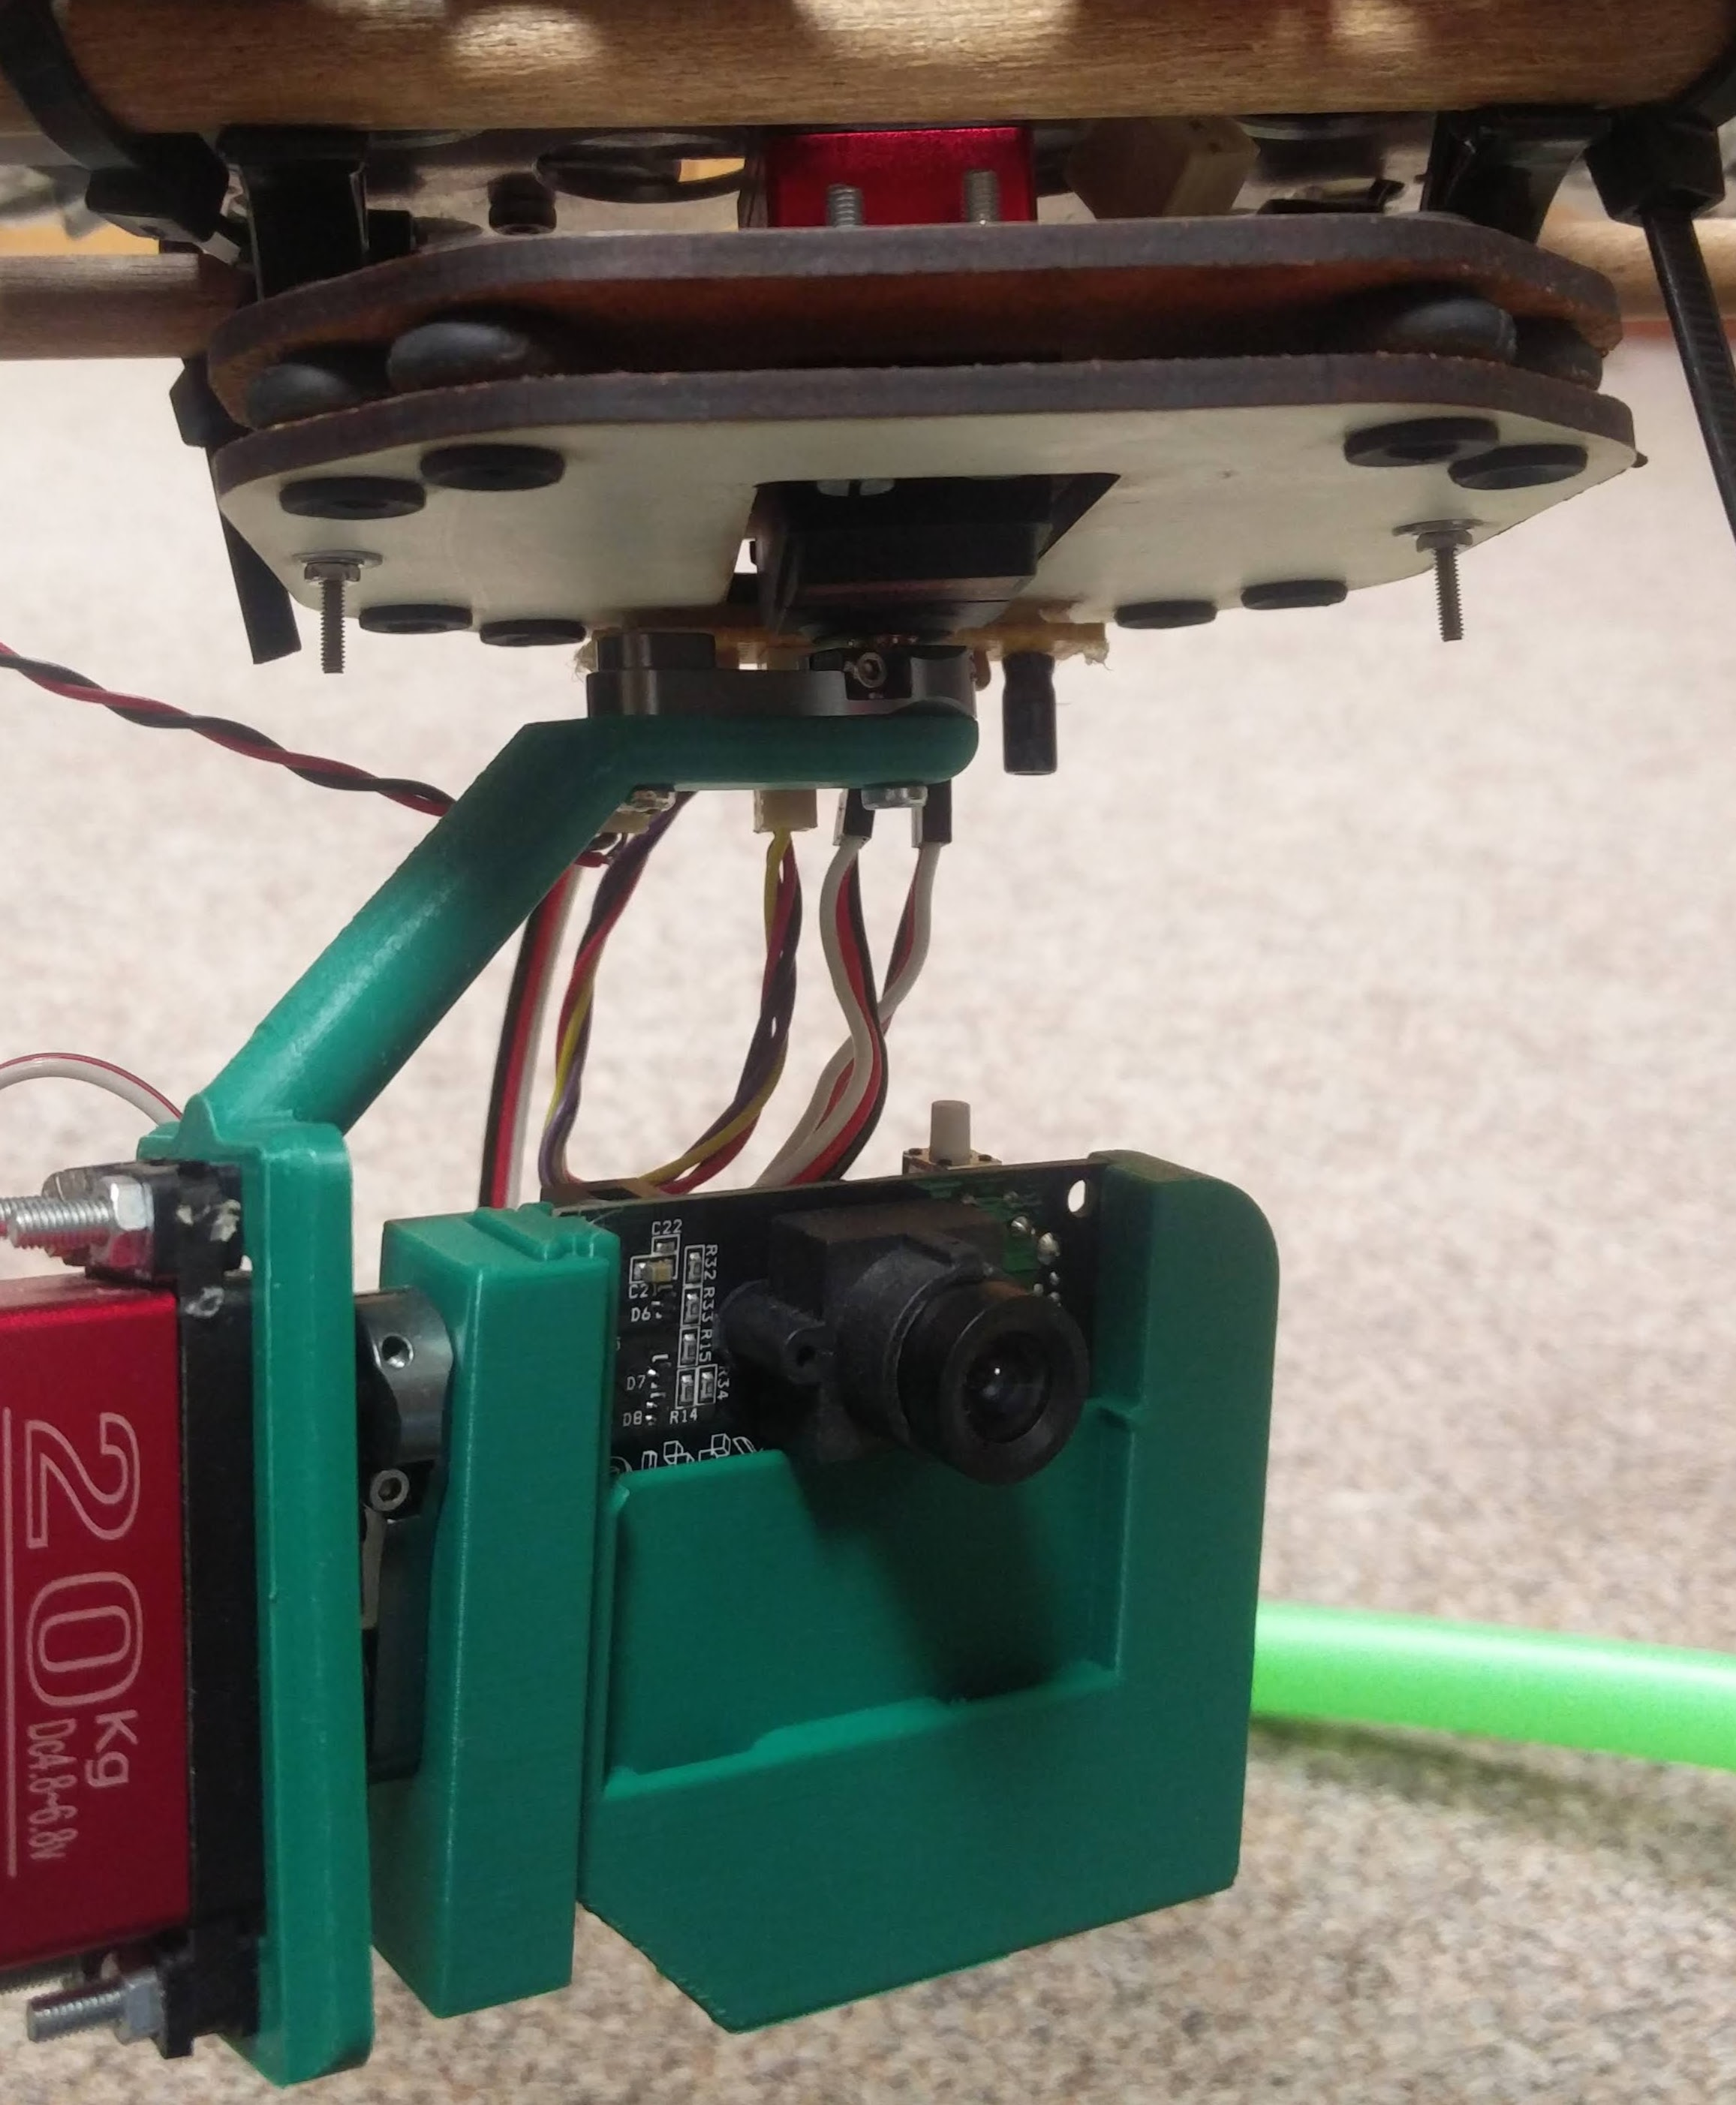
\includegraphics[width=0.4\textwidth]{literature_review/sylvan_gimbal.jpg}
  \caption{\label{fig:sylvan_gimbal} A photo of Sylvan Morris's gimbal design.}
\end{figure}


\subsection{Extended Kalman Filter}
\subsection{Controller design and implementation}


\section{Research Design and Timeline}
\subsection{Research Problem}
narrow angle gopro with computer vision better than multiple wide angled gopros??
\subsection{Elaboration of the Plan of Action}
Do the minimum complete system first, then work on any extras, even if they're core to the idea of the project

Decided that training on cheetahs isn't core



\subsection{Description of activies, methods and software platforms}
python for pretty much all software \\
tensorflow, caffe and keras as DL frameworks \\
git to synchronize work done on pi, my laptop, VM and minibeast \\
extensive use of linux for development



\subsection{... validation}



\subsection{Project Timeline}
January/February: some intro to computer vision stuff. Preliminary research into NCS + initial setup on pi

June/July vac: (forgot exactly)

August/September: work on project

October: final tests, write up thesis, hand in. Also do poster and presentation


%\include{Methodology}
%\chapter{System Modelling and Design}

\chapter{Computer vision implementation}

Having performed a review of literature relevant to the project, it was time to actually build the tracking system.

This chapter describes the steps required to establish a complete computer-vision workflow. Unlike other chapters in this report, it is likely that the software presented here will quickly become outdated - multiple computer vision frameworks are competing for market attention, and changing a lot while doing so \cite{website:comparison_deep_learning_software}. In addition, neural accelerator technology is in its infancy and likely to improve a lot in the coming years. Thus, the section is presented as a general methodology which tries to be independent of framework and branding where possible.

Following this, the actual implementation of the computer vision system is discussed along with some short tests on its performance.

%It should be noted that a lot of mistakes were made in this part of the project - these won't be discussed.

\section{Workstation setup and testing}
Three independent computers were used as part of the complete computer vision workflow - a mid-range GPU-equipped computer to prototype and train neural networks, a regular laptop to test and compile a trained neural network and an small embedded computer which uses the neural accelerator for inferencing.

One software package common among all three computer was git \cite{git}, which was used extensively to keep the files on all three computers synchronized.

\subsection{Setting up a computer for training}
Depending on the selection of computer vision/deep learning framework and the operating system on which it is installed, setting up a computer to train neural networks can range from trivial to extremely difficult. However, there are some commonalities amongst the popular frameworks.

The first step is usually to install CUDA, a GPU-acceleration software developed by NVIDIA for their GPUs \cite{nvidia_cuda}. At the time of writing, most frameworks simply don't support AMD GPUs. Next, install cuDNN, NVIDIA software specifically aimed at increasing performance for deep neural networks \cite{nvidia_cudnn} on their GPUs.

If needed for the deep learning framework, install an appropriate version of python \cite{python}.

Finally, the framework itself should be installed. In this project, three frameworks were tested on Windows.

The first two were TensorFlow and Keras. These are installed using pip, pythons built in package manager. The installation is done by entering the command,\\
\pyth{python -m pip install keras tensorflow-gpu}.

The last package was Caffe. Installation on Windows is difficult due to a lack of support for the OS, and wasn't accomplished during the course of the project.

It should be noted that, if the network will simply be fine-tuned (ie, the network was already trained on a similar dataset and requires minimal further training) then one might actually get away with training the model on a fast CPU.


\subsection{Setting up a computer for testing and compiling}
Most simple tests were run on an easily accessible computer. If using the Movidius NCS, this computer must run a Ubuntu 16.04 as it is the only non-Raspbian desktop OS the Movidius SDK officially supports \cite{website:movidius_install}. Movidius software barely works as is, so it is not recommended to push things even further by messing around with any other OS.

One option is to run Ubuntu on a virtual machine, such as Oracle VirtualBox. If you do this, don't bother trying to make it work with the NCS hardware through the VM - it can be quite tricky getting the drivers to work. Instead, trust that the compiled network will perform as well on the NCS as it does in the uncompiled framework-specific format and save yourself a lot of time.

Next, install the Movidus SDK, as described in the documentation \cite{website:movidius_install}. Despite what the documentation suggests, there isn't a need to \pyth{make} all the examples - this can take a couple hours, use a lot of disk space and not help at all.

After this, the previously trained neural network should be compiled to the Movidius-specific graph format using the \pyth{mvNCCompile} command. If it fails, it is likely that the network has an operation which isn't supported by the Movidius software. To this end it is highly recommended to check whether the operations used in the neural network are supported by Movidius for that particular frame.

If the Movidius SDK installation process has not already done so, it is recommended to install the deep learning framework that will be used. This enables the user to debug their neural network without having access to the inference computer.


\subsection{Setting up a computer for inferencing}
A Raspberry Pi was chosen as the embedded computer that would interface with the neural accelerator. An SSH terminal was used to access it. In order to get it ready for the final platform, some packages needed to be installed - a list of the most relevant python packages not included in a default python installation is as follows:

\begin{itemize}
	\item \pyth{numpy}: a package for fast numerical computing.
	\item \pyth{picamera}: a package to facilitate the use of the Pi Camera module.
	\item \pyth{matplotlib}: a popular plotting library.
	\item \pyth{PIL}: an fast library useful for working with images.
\end{itemize}

These are easily installed by entering the following command in a terminal:\\
\pyth{python -m pip install numpy picamera matplotlib PIL}

Interestingly, it is not actually necessary to install any deep learning framework on the Raspberry Pi. Neither is it necessary to install \pyth{opencv} or even the full Movidius SDK if the neural network has already been compiled to a graph file. Knowing this can save you an absolutely incredible amount of time, as these programs can be incredibly time consuming and frustrating to install. For instance, installing the full Movidius SDK on the Raspberry Pi requires upwards of 10 hours and is prone to failing at almost any point in this installation.

Thus, it is \emph{highly} recommended to instead skip all of these potential issues and rather just install the Movidius SDK in API-only mode \cite{movidius_api_only}. This doesn't take long and is not prone to failure.

Python notebooks were used for all actual programming. In this project, the main advantage to using notebooks was the fact that the notebook server could be port-forwarded to the main development PC, allowing for far easier plotting and visualisation than would be possible using a simpler IDE in an SSH terminal. Note that was important that the code ran on the Raspberry Pi itself to access its hardware, and connect the Pi to an external display would not be ideal as its GPU was needed for other computation.


\section{Selection of computer vision framework}
At the time of writing, the Movidius NCS only supports the TensorFlow and Caffe machine learning frameworks \cite{website:movidius_install}. Based largely on its popularity and ease of use, TensorFlow was chosen as the architecture which would be used for the project \cite{website:tensorflow_popularity}. However, TensorFlow is quite low-level and provides fairly slow and inconvenient methods of model creation, training and testing. It certainly has advantages but ease of development is not one of them.

To combat this, another option is to instead use Keras, a deep learning library which provides a far more intuitive interface. It allows the user to specify which backend they'd like to use for the actual number crunching. Among other options, one of the available backends is TensorFlow. The popularity of Keras has grown to such an extent TensorFlow has incorporated it as an official API.

The plan was then to retrain a neural network (possibly after modifying it) using Keras, export the model architecture and weights in TensorFlow format, and then compile it down to the Movidius NCS graph format. The hypothesis was that while researchers often aim to create neural networks which can classify more and more types of classes at once, this project only required up to three: cheetahs, humans and dogs. This meant that useless parts of the network (neurons which never fire as they aren't needed) could potentially be removed \cite{molchanov2016pruning}. This process is known as 'pruning', and can significantly decrease inference time.

However, after far, far too much frustration, it was discovered that the support for each framework was far from equal. Networks created in TensorFlow quite consistently failed to compile. After examining the Movidius documentation more closely, it was discovered that the number of operations supported for TensorFlow was simply far smaller than the number supported for Caffe. For instance, the TensorFlow \pyth{concat} operation doesn't appear on the list of compilable operations. This left Caffe as the only other available framework.

\section{Selection of CNN architecture}
By this stage, the work spent on object detection had exceeded time estimates and was threatening to compromise the time available for the other components in the system. In addition, Caffe has extremely poor support for Windows machines and no there were no dedicated GPU-enabled Linux PC was available for use as a neural network training machine. For these reasons, it was decided the an unmodified pretrained Caffe model would be used.

%https://github.com/movidius/ncappzoo/tree/master/caffe
In order to mitigate further risk of a model not working correctly on the NCS, only architectures with official support from Movidius were considered. At the time, this narrowed the choice down to a single option: SSD MobileNet, the combination of MobileNet and SSD, two independently designed neural network architectures.

MobileNet is a class of image classifiers designed by researchers at Google \cite{arXiv:1704.04861}. Since it was designed for mobile devices, it trades some classification accuracy for performance. However, the architecture is remarkable in that the performance increase is usually significant while the classification accuracy decrease is not. It acts a feature extractor in this particular model.

SSD (short for Single Shot MultiBox Detector) is a an object detector \cite{arXiv:1512.02325}. When used with another network as a feature detector, it takes in features, scales them to a variety of sizes and finally, after some more processing, outputs a vector which embeds information on the number of objects found, the predicted class for each object, pixel coordinates of the bounding box around each object and a number from 0 to 1 which represents the confidence in the network's prediction. Hence, the name - a single pass through the network resulting in the detection and boxes of multiple objects.

As a backup, another option would have been to perform the sliding window technique using an image classifier. There could be merit to this: a clever algorithm might first search parts of the image where it expects to find the object, reducing the overall computational requirements.


\section{Implementation of computer vision system}
Once all required software packages were installed, the next step was to start integrating the various components in the computer vision pipeline.

\subsection{The Raspberry Pi camera}
For the sake of convenience and low latency imaging, it was decided that a Raspberry Pi v2 camera module would be used to provide a stream of photos for the CNN. The camera plugs into a Raspberry Pi using a flat ribbon cable, as shown in Figure~\ref{fig:r_pi_camera}.

\begin{figure}[h!]
  \centering
  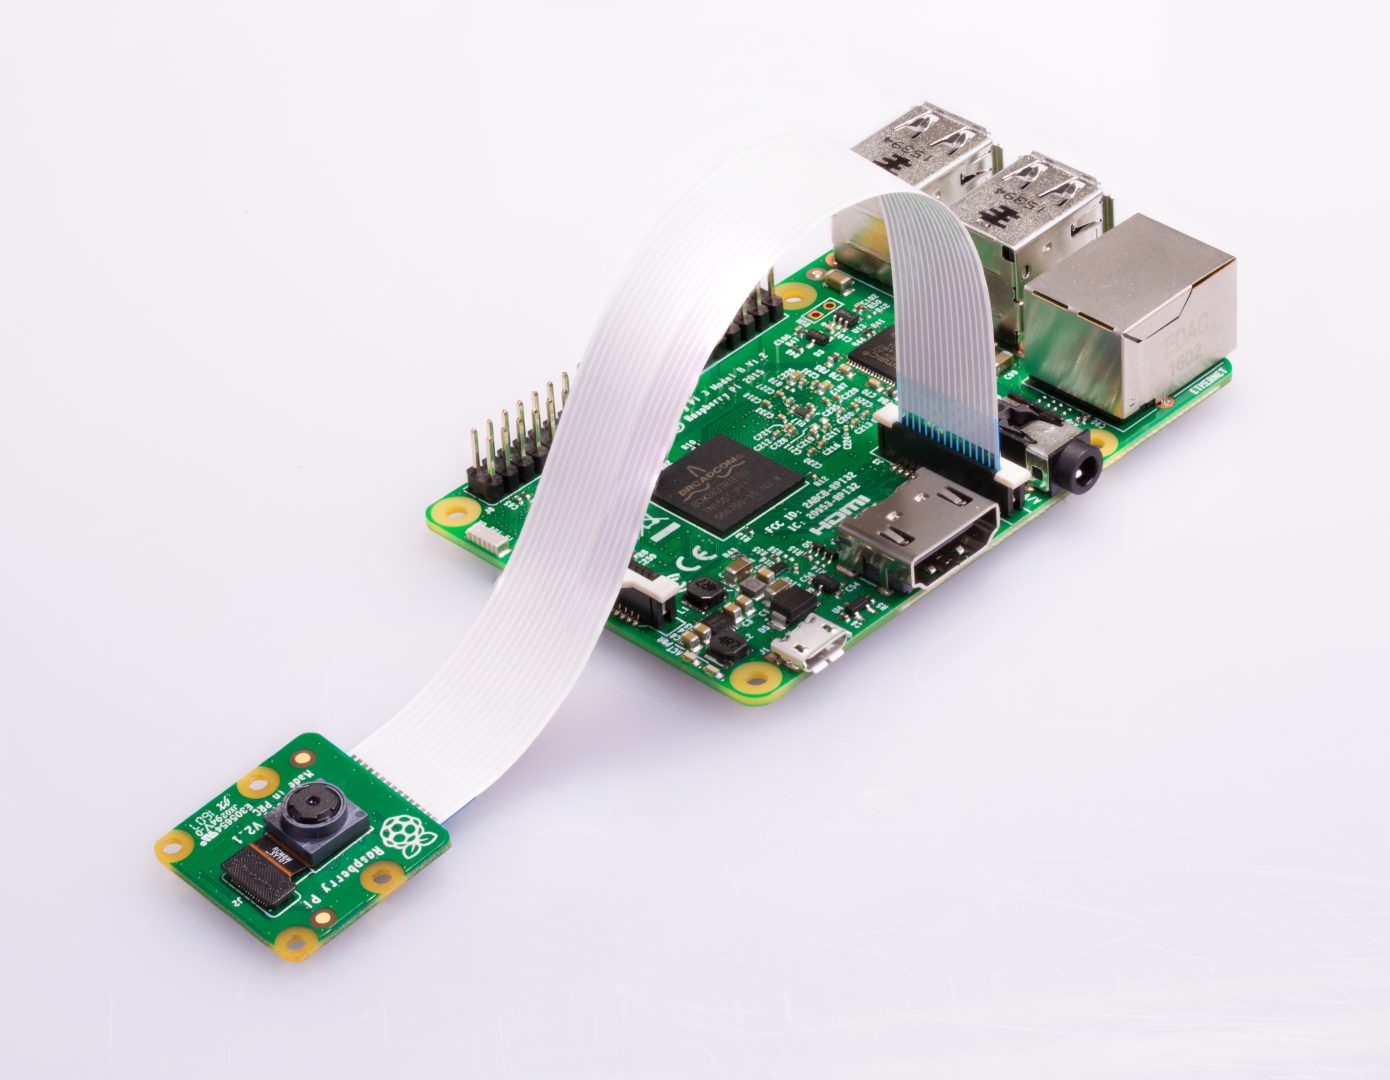
\includegraphics[width=0.5\textwidth]{methodology/r_pi_camera}
  \caption{\label{fig:r_pi_camera}A photo of a Raspberry Pi connect to a Raspberry Pi camera module.}
\end{figure}

An alternative would be to attempt to stream from the GoPro cameras themselves, but this would result in a higher latency as the photos have to be transferred via WiFi and would not use the Pi's built in hardware encoding \cite{website:gopro_to_rpi, website:gopro_to_rpi2}.

As described in the excellent \pyth{picamera} module documentation \cite{website:picamera_hardware}, one must be careful about selecting a sensor mode and camera resolution which makes use of the full FOV available (62.2\textdegree $\ \times$ 48.8\textdegree). Lower resolutions and fast sensor modes tend to take a simple crop of the centre of the image (reducing the FOV) instead of taking a full photo and resizing it. The price paid for this is latency - the higher the resolution, the more data flows through the pipeline and computation must be done.

A resolution of \pyth{1640 x 1232} maximised the FOV. Since the Pi Cameras sensor resolution is \pyth{3280 x 2464}, it uses 2$\times$2 binning to easily achieve this downscaling. Next, the Pis GPU was used to easily resize the image down to \pyth{320 x 304} - only a few resolutions are support by the library and this one was close to the resolution typically used by CNNs, so further resizing on the Pis CPU would require minimal processing time.

Finally, the video port was used to take photos instead of the camera. This was done to decrease latency - while both the video port and still port constantly send photos down the ribbon cable to the pi, using the video port results in less anti-noise post-processing (and thus lower latency).

%As is normal in Python, once the exact problem had been understood, the solution in code was relatively straightforward. The following code is enough to set up the pipeline mentioned thus far: \\ \\ \\ \\

%\begin{python}
%with picamera.PiCamera(resolution=(1640, 1232),
%                       framerate=40,
%                       sensor_mode=5) as camera:
%     # (320, 304) is closest to neural network input of (300,300)
%    frame = picamera.array.PiRGBArray(camera,
%                                      size=(320, 304))
%    # use GPU for resizing - will resize to nn_shape later
%    cont_capture = camera.capture_continuous(frame, 'rgb',
%                                             resize=(320, 304),
%                                             use_video_port=True)
%\end{python}

%After this, a simple function call of \pyth{next(cont_capture)} would fetch the latest frame from the continuous stream of photos, perform some post-processing and then place it in the \pyth{frame} buffer, where it could be accessed using \pyth{frame.array}.

\subsection{Compiling a trained neural network}
A trained SSD MobileNet was found on GitHub user chuanqi305's \href{https://github.com/chuanqi305/MobileNet-SSD}{online git repository} \cite{website:chuanqi305_nn_github}. It has an input dimension of $300 \times 300 \times 3$, and was largely trained on MS-COCO before being fine-tuned on VOC0712 (MS-COCO and VOC0712 are two large, freely available datasets \cite{website:mscoco_dataset, website:voc2012_dataset}). It was trained to predict make predictions for 20 classes, including 'person', 'dog' and 'cat'. The reason for choosing a network which predicted these classes, was because tests would be done on (easily accessible) humans and dogs. In addition, if the network was to be retrained to detect cheetahs, starting from detecting cats or dogs might help decrease training time and the amount of data required.

After confirming that the license for usage of the model is permissive, it was downloaded and then compiled on a windows laptop running an Ubuntu VM with the full Movidius SDK installed, using the \pyth{mvNCCompile} command. The graph file was then transferred to the Raspberry Pi via an ssh terminal.

Using Movidius code from tutorials as a starting point, the graph file was uploaded to the NCS. The camera module presented above was then used to take a photo and store it as an array of unsigned 8-bit integers (integers from 0 to 255).

The CNN used required some preprocessing before an image could be passed in as an input. Specifically, the images should be represented as an array of floats with a mean of 0 and a range of $(-1, +1)$. This was done using the calculation,%\\ \\

\begin{python}
mean = (127.5, 127.5, 127.5)  # 3 colour channels, 255/2 == 127.5
scale = 1/127.5
preprocessed_img = (img - np.float32(mean)) * np.float32(scale)
\end{python}

Pre-processed images were then sent to the NCS, which passed them through the CNN in a time of about 80 ms. The serialized output of SSD network was then decoded into a python dictionary which contained easy to manage information about the objects in the frame.

\section{Testing the computer vision model}
The next step was to test the data pipeline created thus far. The main issues being tested were,

\begin{enumerate}
\item The general classification accuracy of of the network,
\item The extent to which the predicted position overlaps with the actual position,
\item How blurry/dark/out of focus the image can be before the network stops working, and finally,
\item The inference time of the network, with and without the NCS.
\end{enumerate}

Code to redo these tests can be found on the authors \href{https://github.com/alknemeyer/EEE4022S-Thesis-Project/blob/master/Final%20code/tests.ipynb}{GitHub repository}.


\subsection{Accuracy of the predictions}

The setup was tested by passing photos through the neural network, and then superimposing the predicted bounding box output onto the image along with a text description of the predicted class. A measure of confidence (written as a percentage by convention, but not actually a statistical measure) was also added to show how trustworthy the prediction was.

First, a photo of the author's dog was tested. The network correctly predicted 'dog' with a high confidence measure of 99\%. This is shown in Figure~\ref{fig:box_around_blossom}.

\begin{figure}[h!]
  \centering
  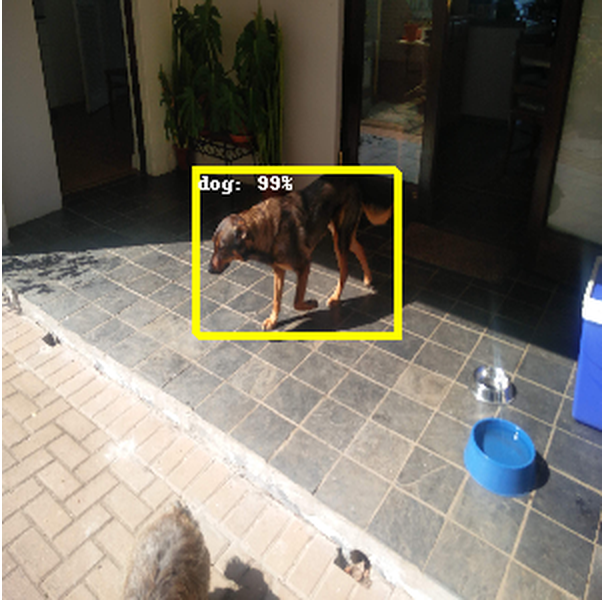
\includegraphics[width=0.7\textwidth]{methodology/box_around_blossom}
  \caption{\label{fig:box_around_blossom}A photo of the authors dog, correctly predicted with 99\% confidence.}
\end{figure}

Next, three images of the author were tested. They are shown in Figures~\ref{fig:box_around_me_crouching}, \ref{fig:box_around_me_running} and Figure~\ref{fig:box_around_people_hard}.

\begin{figure}[h!]
    \centering
    \subfloat[][A photo of the author while crouching, correctly predicted with 88\% confidence.]{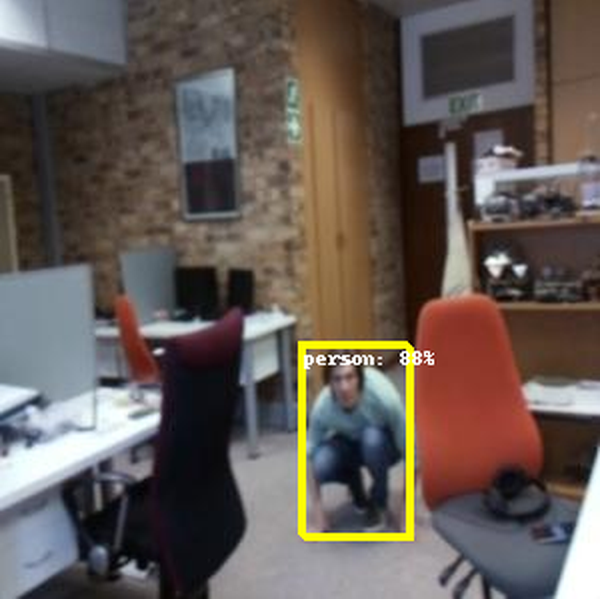
\includegraphics[width=0.48\linewidth]{methodology/box_around_me_crouching}\label{fig:box_around_me_crouching}}
	\quad
    \subfloat[][A photo of the author while running, correctly predicted with 96\% confidence.]{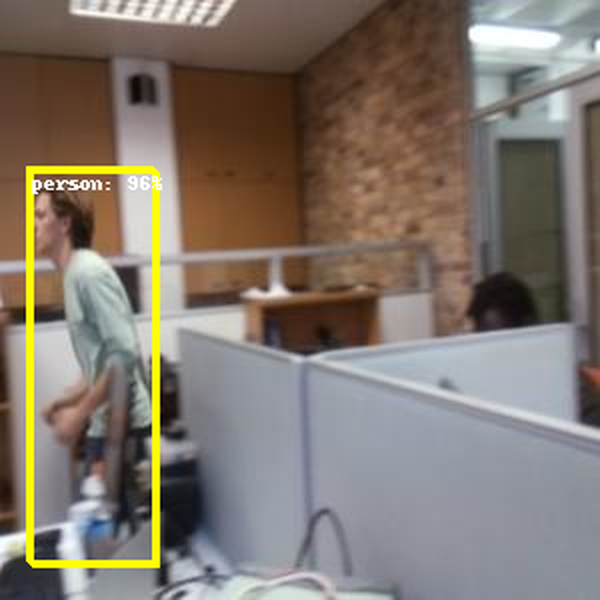
\includegraphics[width=0.48\linewidth]{methodology/box_around_me_running}\label{fig:box_around_me_running}}
    \caption{Photos of the author looking silly while moving around a laboratory.}
\end{figure}

Figures~\ref{fig:box_around_me_crouching} and \ref{fig:box_around_me_running} show that the neural network can correctly classify objects in non-standard positions (such as when the classified object is in a crouch position, or from the side) in relatively complex environments, such as a laboratory with textured brick walls. The camera was moved slightly during both of the photos, resulting in slightly blurred images. This was done to emulate the gimbal moving the camera system. The confidence ratings were 88\% and 96\% respectively.

The final image, shown in Figure~\ref{fig:box_around_people_hard}, was a bit of a surprise in that the network far surpassed the authors expectations.

\begin{figure}[h!]
  \centering
  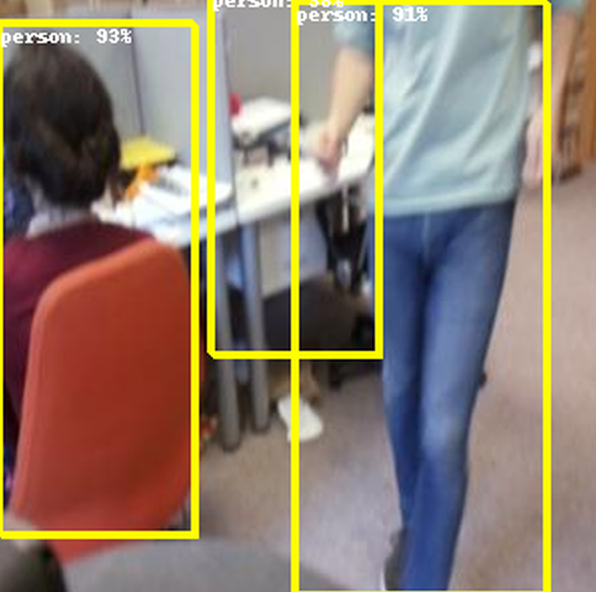
\includegraphics[width=0.5\textwidth]{methodology/box_around_people_hard}
  \caption{{\label{fig:box_around_people_hard}A photo of a person sitting and the bottom two thirds of another person standing, correctly predicted with 93\% and 91\% confidence respectively.}}
\end{figure}

Two people were correctly identified: a woman at a desk in the left of the frame with a confidence of 93\%, and the bottom two thirds of the author on the right side with a confidence of 91\%. Faces have been one of the easiest things to detect in computer vision \cite{website:face_detection_survey}, so it was a pleasant surprise to find that the network doesn't need a face at all.

There was also a false-positive detection in the centre of the frame. However, the confidence for this detection was 38\% - low enough that the recommended confidence threshold of 70\% confidence \cite{website:chuanqi305_nn_github} would have resulted in it being ignored.% \\

\subsection{Observed performance increase due to NCS}\label{ssec:meth_nn_performance_increase}
Next, the performance increase of the NCS was tested to confirm that the device was in fact necessary. For the purposes of the tests, the pre-processing time and latency of the camera were ignored as they are common to all methods of inferencing. It is worth noting that there will always be variability when timing the runtime of a process on a non-realtime OS using a language which occasionally pauses for garbage collection.

First, the Pi was tested on its own. Using the CPU, roughly a full second was required to get from pre-processed image to serialized results. Due to multithreading, up to four images may be processed side by side (staggered 250ms apart) for a total sampling rate of 4 Hz with a latency of 1 second.

Next, the Pi was tested with the Movidius NCS. It took around 20 ms to send the image to the devices memory, and then around 80ms to receive the result. The NCS can't process multiple images simultaneously, so this equated to a speed of 10 Hz with a latency of 100ms.

This proved that, short of using another form of CNN acceleration, the NCS was vital to the project's success.


\chapter{Gimbal design}

Since the camera system must be able to track an object, a gimbal was required rotate the payload: two small HD cameras, a distance sensor and the raspberry pi cam used for tracking.



\chapter{EKF Modelling and Design}

\section{System modelling}
An EKF was used to estimate the state of the tracked object as it moves around. Since the camera system generally rotates around an axis and there is no reliable estimate of the distance from the camera to the object being tracked, it was decided that the state would be measured in angular coordinates.

A model of the dynamics of the tracked object had to be chosen for the EKF to operate optimally. However, there is no possible "correct" model for the movements of the object being tracked (for example, a cheetah won't stick to the rule of moving at a constant velocity) and no way to estimate the disturbances $u$ which may effect its decision to change its velocity. Thus, it was decided that the model would make the incorrect assumption the the object would either maintain a constant velocity, constant acceleration of exponentially decaying acceleration. These three approaches needed to be tested, with the best being used in the final model.

This resulted in the global angular position, velocity and acceleration of the tracked object were estimated. These were stored in the state matrix $x$ as,

\[ \underline{x} = \begin{bmatrix} \theta \\ \dot{\theta} \\ \ddot{\theta} \end{bmatrix} \]

These states are related through integration, where $\theta = \int{\dot{\theta} dt} = \int{\int{\ddot{\theta} dt}dt}$. The can be approximated using the discrete integration formulae, $\dot{\theta}_k = \dot{\theta}_{k-1} + \Delta T \ddot{\theta}_{k-1}$ and $\theta_k = \theta_{k-1} + \Delta T \dot{\theta}_{k-1}$. The prediction matrix was thus chosen as,

\[ F = \begin{bmatrix} 1 & \Delta T & 0 \\
                       0 & 1 & \Delta T \\
					   0 & 0 & \beta
		\end{bmatrix} \]

where $\beta$ is a factor which could be $\beta = 1$ for constant acceleration ($a_i = a_{i-1}$ in the predict stage), $0 < \beta < 1$ for decaying accelerating (for example, $a_i = 0.9 a_{i-1}$) or $\beta = 0$ for no acceleration. This was done to ensure quick and easy prototyping.

Next, the sensor needed to be added. The neural network returns the coordinates of the position of the object, measured in pixels. For the sake of modularity and simpler math, the pixel range of \pyth{pixel} $\in$ \pyth{[0, 299]} along a single axis was normalized to a value \pyth{pixel_norm} $\in$ \pyth{[-1, 1]}, with a pixel value of zero corresponding to the centre of the image. An illustration of this is shown below, in Figure~\ref{fig:pixel_to_angle}.

\begin{figure}[h!]
  \centering
  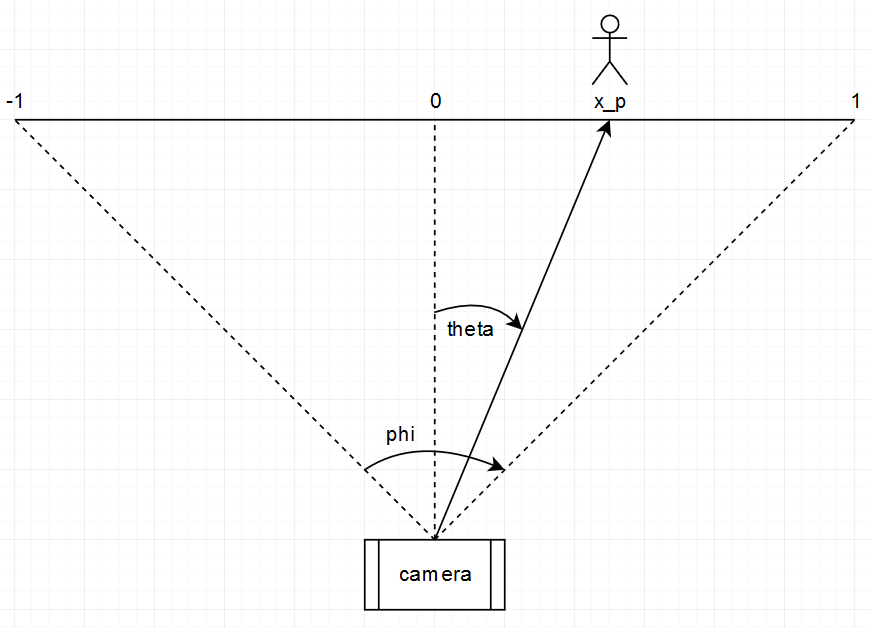
\includegraphics[width=\textwidth]{methodology/pixel_to_angle2}
  \caption{\label{fig:pixel_to_angle} Diagram showing the mapping from normalized pixel to angle.}
\end{figure}

Note that the pixel coordinate of the detected object is given by \pyth{x}, the angle to the object is \pyth{phi} ($\phi$) and the field of view of the camera is \pyth{theta} ($\theta$). Letting the distance between the camera and the plane at the closest point be noted as $L$, one can convert between pixel and angle as follows:

\[ L = \frac{1}{\tan{\theta/2}} = \frac{x}{\tan{\phi}} \]
Resulting in,
\[ \phi = \tan^{-1}{\left( \frac{\tan{ \theta/2 }}{x} \right) }
\qquad or
\qquad x = \frac{\tan{\phi}}{\tan{\theta/2}} \]

Thus, the mapping from pixel to angle is nonlinear. This is why an EKF was chosen instead of a linear Kalman Filter - a one pixel error in the middle of the image will propagate to a different angular error than a one pixel error at the edge. The Jacobian could then be calculated as,

\[ \frac{\delta h}{\delta x} = \frac{\delta}{\delta x} \left[ \frac{\tan{\phi}}{\tan{\theta/2}} \right] = \frac{1 + \tan{(\phi)}^2}{\tan{\theta/2}} \]

Finally, the $Q$ and $R$ matrices needed to be determined. In most systems, these can be calculated after careful modelling of the objects dynamics and consultation with component datasheets. However, in this system, the $Q$ matrix determined for an object which is close to the camera would be wildly inaccurate when the object is farther away, since distance affects the perceived angular movement of an object moving in a straight line. Since there is no distance estimate, this could not be reliably factored into a constantly changing $Q$. In addition, the neural network has no obvious value to use for the sensor noise, $R$.

Thus, it was decided that these would be left as parameters to be tuned using recorded data.

\section{Implementation of the EKF}

While python wasn't designed for purely numerical programming (such as matrix multiplication), when the correct packages are used it can approach C-level speeds. \pyth{numpy} is one such package - it provides python bindings to C arrays, resulting in incredible speedups over regular python arrays.

Thus, the Kalman Filter and Extended Kalman Filter were implemented as python classes which contain \pyth{numpy} matrices. A snippet of the implementation can be seen below, while the rest of the code can be found on the author's GitHub page. \\

\begin{python}
class KalmanFilter():
    def __init__(self, Ts, Q, R, a=1):
        self.Ts = Ts
        self.x = np.matrix([[0],  # position
                            [0],  # velocity
                            [0]]) # acceleration
        self.P = np.matrix(np.eye(3))
        self.F = np.matrix([[1, Ts,  0],
                            [0,  1, Ts],
                            [0,  0,  a]])
        self.Q = np.matrix([[Q*(Ts**2),    0, 0],
                            [        0, Q*Ts, 0],
                            [        0,    0, Q]])
\end{python}

\section{Tuning the process noise and sensor uncertainty}
The next step was to find and set reasonable values for the process noise $Q$ and sensor uncertainty $R$. This was doing by running the computer vision algorithm while a human walked and ran around the lab. The results of this were saved to a file, allowing for easy offline simulation. A plot of the raw updates from the neural network are shown below, in Figure~\ref{fig:raw_nn_results}.

\begin{figure}[h!]
  \centering
  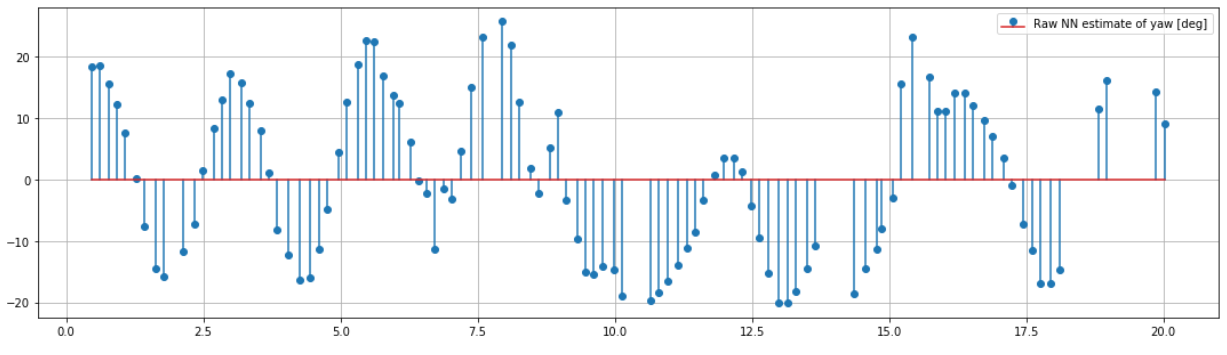
\includegraphics[width=\textwidth]{methodology/raw_nn_results}
  \caption{\label{fig:raw_nn_results} A plot showing the outputs of the neural network, and the timing thereof.}
\end{figure}

Note how the time between inferences from the neural network is not constant - while all of the calculations in the neural network are the same in each run, non-constant run times are the natural consequence of running a control loop on a non real time operating system and using a programming language which stops occasionally for garbage collection.

In addition, there are times when a few hundred milliseconds pass without receiving a new update - this occurs when the neural network can't find an object in the frame. It is worth noting that the neural network is in fact very good at locating objects, and misses them infrequently. However, the frequent and large gaps in object locations was added in order to simulate tracking an object which may disappear behind a bush or some other obstacle.

Next, a small script was made to speed up the trial-and-error process of comparing the advantages and disadvantages of a variety of $Q$ and $R$ values. In addition, the possibility of switching to a Kalman Filter and changing the acceleration modifying parameter $\beta$ were added. In the end, values were chosen to satisfy the following two criteria:

\begin{enumerate}
\item Trust the updates from the neural network more than the model itself. This was decided on because the network was known to accurately find objects in a frame, whereas the constant velocity or acceleration model was \emph{known} to be incorrect.
\item Make reasonable predictions in the event that no updates appeared from the neural network. 'Reasonable' meant that, if the data indicated that the object was moving in a certain direction at a certain velocity, it is reasonable that the object would keep moving in that direction and at that velocity.
\end{enumerate}

A plot of the interactive process and selected paramters is shown below, in Figure~\ref{fig:tuning_Q_R}.

\begin{figure}[h!]
  \centering
  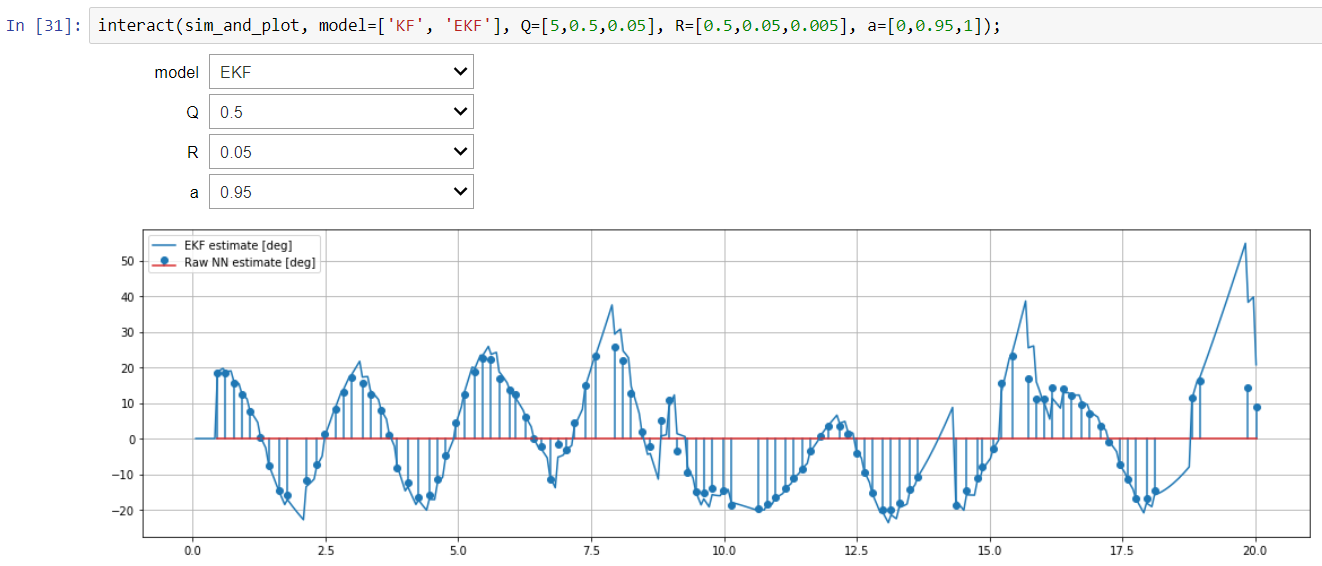
\includegraphics[width=\textwidth]{methodology/tuning_Q_R}
  \caption{\label{fig:tuning_Q_R} A plot of the output of the EKF given stem plot data as input.}
\end{figure}

As can be seen in Figure~\ref{fig:tuning_Q_R}, choosing $Q = 0.5$, $R = 0.005$ and $a = 0.95$ resulted in an EKF which closely follows and trusts the updates from the neural network, whilst making reasonable predictions in the event that no data was received. It is worth noting that the input data was more sinusoidal than 'roughly constant velocity', which was the main assumption behind the dynamics of the model. This was due to a lack of running space in the mechatronics engineering lab - once wall has been reached, there's no place to go except backwards.

This concluded the implementation of the Extended Kalman Filter.

\chapter{Control Loop Design and Implementation}

\chapter{Results}

\chapter{Discussion}\label{chap:discussion}

Some things should be noted when considering the results shown previously.

The first is that, unless one decreased the effects of the image recognition latency, an angle between the cameras orientation and the object will always remain. This can be diminished if one has better knowledge of the animals movement prior to the experiment - for example, if it was known that the only thing being tracked is an object moving from left to right, the yaw Kalman Filter would be able to more reliably predict the current position of the object based on delayed data. This could result in better tracking, but comes with its own problems (such as overshoot if the object slows down).

The second issue to discuss is that of the maximum angular range of the system, which is limited only by the wiring connecting the stationary part of the tracker to the rotating parts. While the tracker itself has a maximum angular rotation width of 140\textdegree, a portion of the field of view of the camera could be added to this. It may not make sense to add the full width, since part of the premise of the tracker is that object is aimed at directly.

Another topic is the tracking speed of the gimbal, and how it failed to track objects with high a velocity or acceleration. The Kalman Filters noise parameter can be adjusted to vary the state estimate from smoothness as a priority (which could be interpreted as seeing sudden changes in the sensed position as noise, which should be rejected) to robust tracking as a priority (where a sudden change in state is seen as quick movement). In addition, the system would sometimes be unable to track a fast moving object simply due to the gimbals slower rotational rate, which wasn't investigated in time. It is unclear whether the Kalman Filters parameter or gimbals slow movement contributed more to the poor performance in this regard.

Finally, all of the tests were performed in a relatively confined space tracking close objects. It is unclear how well the tracker would perform tracking faster objects further away. However, based on the results of this report, one could estimate its performance using the formula $\omega = v/r$, where $\omega$ is the rotational velocity, $v$ is the tangential angular velocity and $r$ is the distance to the object. Since the object tracker is confined to track objects at a certain maximum angular rate, but objects themselves move with linear velocities, as long as $\omega$ remains constant between tests on a human in a lab and a cheetah outdoors it is likely that the system would continue to track well.

\chapter{Conclusions}

Based on the test results shown in Chapter~\ref{chap:results} and discussion in Chapter~\ref{chap:discussion}, it can be conclusively said that the tracking camera system works better than a stationary camera setup. This is due to three main reasons:

First, the maximum field of view of the tracking system is significantly greater than that of a single stationary camera. One could use multiple stationary cameras, but this comes at a higher cost and extra work on the part of the researchers.

Second, the distortion which arises from setting the stationary cameras to wide-angle mode is significantly higher than the distortion from setting the tracking cameras to an narrow angle mode. One could counter this buy purchasing even larger numbers of stationary cameras and setting each to the less distorting narrow field of view, but this comes at a higher cost and with extra work on the part of the researchers.

Third, there are other benefits to having a system which aims at a target which aren't practically feasible using a stationary camera setup. For instance, one could attach one or more distance sensors and a GPS to the gimbal to estimate the absolute location of the object.

When viewed as a general tracker in its own right, it is clear that the system is not perfect and could see significant benefits given an extra week or two of time. The study was also not conclusive in that the tests in the laboratory alone aren't enough to empirically prove that the system could track a fast moving cheetah (given a neural network which can detect one). 

\chapter{Recommendations}

ideas:
\begin{itemize}
	\item track global x,y coordinates of cheetah. Requires depth estimating nn or distance sensor (tricky because you aren't always point at cheetah). Other option is to your height and elevation to estimate the distance
	\item get a faster camera (higher FPS)
	\item faster SBC
	\item 3-axis gimbal
	\item avoid movidius, if possible
	\item add encoder to gimbal or offset camera to avoid lining up accelerometer axis with rotation axis
	\item consider switching away from python to an even faster language with less garbage collection problems - for example, julia. Can also be low-level, now that most of the debugging/prototyping has already been done.
\end{itemize}

%\include{References}
\appendix
%\include{appendixa}
%\include{appendixb}

\bibliographystyle{plain}
\bibliography{references}
{\Large \color{red} find out how to include the url}

}
\end{document}
